

\section{Recolección de datos}

En esta sección describiremos el proceso de recolección de datos. La salida de esta etapa será un conjunto de artículos y sus comentarios extraídos de Twitter. Describiremos a continuación las decisiones realizadas respecto a las fuentes y a decisiones técnicas realizadas.

\subsection{Diarios elegidos}

Limitamos nuestra recolección de datos a cuentas de diarios de la República Argentina y, puntualmente, nos centramos en diarios con comunidad mayormente rioplatense ya que (como comentaremos más adelante) los anotadores son nativos de esa variedad dialectal. Esto es teniendo en cuenta que esta tarea depende fuertemente de la jerga y de las variaciones dialectales de cada país decidimos realizar sólo anotación de estos diarios.

Además, si bien buscamos otros medios del interior (como por ejemplo ``La voz del Interior'', diario dirigido mayormente a un público fuera de la Metrópolis de Buenos Aires) observamos que la interacción en Twitter de estos medios es muy baja: pocos usuarios comentan sus notas. En pos de maximizar

Los diarios seleccionados fueron los siguientes:

\begin{itemize}
    \item @infobae
    \item @clarincom
    \item @perfilcom
    \item @LANACION
    \item @cronica
\end{itemize}


Si bien recolectamos notas de otros medios, no los consideraremos a partir de ahora, y los dejamos para análisis posteriores. Los medios elegidos son medios formales y tradicionales, la mayoría de ellos con soporte escrito. Consideramos la posibilidad de elegir medios no tradicionales y más orientados a grupos de la derecha ``alternativa'' (puntualmente, ``La Derecha Diario''\footnote{\url{http://twitter.com/laderechadiario}}). Estos medios son altamente generadores de contenido de odio. Sin embargo, finalmente tomamos la decisión de descartarlos de las subsiguientes etapas.


\subsection{Método de recolección}



La API de Twitter\footnote{Usamos la versión 1.1 de la API. La versión 2.0 parece facilitar la recopilación de conversaciones} en su versión gratuita, nos brinda dos modos de recolectar tweets de su plataforma:

\begin{enumerate}
    \item Search API: permite buscar tweets en base a términos, de hasta 15 días atrás sobre una pequeña muestra, recreando lo que vemos en la UI de Twitter
    \item Stream API: permite buscar tweets en tiempo real sobre una muestra de cerca del 1\% de todos los tweets de la red social
\end{enumerate}

La API Stream, mientras por un lado limita temporalmente la recolección de datos, por el otro nos brinda la posibilidad de recolectar una mayor cantidad de información en tiempo real. Más aún, dada la naturaleza de nuestros datos (discurso de odio), se corre el riesgo de que con el tiempo sean moderados e inaccesibles para cualquier búsqueda con la API Search. \todo{Mencionar algo de los términos y condiciones de Twitter}


Por lo explicado, usamos la API de Twitter Stream mencionando cualquiera de estas cuentas. Si estamos entonces recolectando tweets sobre \verb|@medio|, el proceso de recolección nos da:

\begin{enumerate}
    \item Tweets de \verb|@medio|
    \item Respuestas a los tweets de \verb|@medio|
    \item Tweets de terceros que mencionan a \verb|@medio|
    \item Retweets (RT) de tweets de \verb|@medio|
    \item Citas de tweets de \verb|@medio|
\end{enumerate}

Los RTs y tweets que arroben a \verb|@medio| carecen de interés para nuestro estudio, con lo cual los descartamos. Por otro lado, también descartamos las citas, aunque podrían entenderse como ``respuestas'' a los tweets originales. Nos quedamos con tweets de \verb|@medio| y las respuestas a estos. Si bien la API nos da estos tweets desestructuradamente, reconstruimos el árbol de la discusión mediante el campo \verb|in_reply_to_status_id|\footnote{Ver la documentación y la referencia al campo en \url{https://developer.twitter.com/en/docs/twitter-api/v1/data-dictionary/object-model/tweet}}.

Para el propósito de este trabajo, solo estamos interesados en el primer nivel de respuestas al tweet original, y no incorporaremos hilos de respuestas.

También eliminamos las URLs de los artículos de los enlaces.




\begin{table*}[t]
    \centering
    \begin{tabular}{ c|c|c }
        coronavirus  &  encierro          & síntomas \\
        covid        &  fase              & fiebre   \\
        cuarentena   &  infectados        & distanciamiento     \\
        normalidad   &  Wuhan             & aislamiento\\
    \end{tabular}
    \caption{Palabras usadas para recolectar artículos relacionados a COVID-19.\label{tab:article_words}}
\end{table*}


Accidentalmente, la recolección de datos se dio al mismo tiempo del estallido de la pandemia del COVID-19. Por ese motivo, y dadas las implicancias de la pandemia sobre el discurso discriminatorio en las redes sociales, se hizo foco en artículos relacionados con COVID-19. Para ello, seleccionamos artículos buscando una cantidad de palabras en su cuerpo, por lo que seleccionamos específicamente artículos relacionados con COVID-19. La tabla \ref{tab:article_words} contiene las palabras utilizadas para recuperar estos artículos.

\subsection{Datos recolectados}

\begin{table}[t]
    \centering
    \begin{tabular}{l|c|c}
    Medio      & \#Artículos & \#Comentarios \\
    \hline
    @infobae   &  45,652   &  822,462 \\
    @clarincom &  29,050   &  672,401 \\
    @perfilcom &  8,764    &  61,203  \\
    @LANACION  &  16,040   &  506,091 \\
    @cronica   &  17,250   &  70,872 \\
    \hline
    Total      & 116,756  & 2,133,029 \\
    \end{tabular}
    \caption{Artículos recoletados por medio}
    \label{tab:articulos_recoletados_por_medio}
\end{table}


En la tabla \ref{tab:articulos_recoletados_por_medio} damos los números de los artículos recolectados por cada medio, luego de aplicado. Si bien recolectamos más artículos de otros medios, no son enumerados. Infobae es el medio que más producción de artículos genera, y también será finalmente sobre el que más comentarios etiquetemos.

La figura \ref{fig:fecha_articulos_por_medio_todas} muestra la distribución temporal de los artículos, sin aplicar ningún filtro por palabras, mientras que \ref{fig:fecha_articulos_por_medio_covid} muestra aquellas relacionadas al COVID-19 utilizando el filtro de palabras listado en la tabla \ref{tab:article_words}. Podemos observar dos caídas. Hay un pequeño pozo en mayo 2020 que se debió a la caída de nuestros servidores de recolección. Por otro lado, observamos que algunos medios (particularmente La Nación) parecieran mencionar menos directamente al COVID (al menos con los términos referidos anteriormente) hasta un nuevo pico cerca de fin de año, coincidente con un nuevo rebrote del virus en este país.

Sin embargo, todo esto puede ser un artefacto del método de filtrado: muchas notas contienen links a otras con sus títulos y eso puede interferir en estas estimaciones. Así y todo, decidimos mantener este método ya que consideramos que mayormente las notas en el período referido tienen relación con la pandemia.

Si bien en las siguientes secciones realizaremos un filtrado de la mayoría de estos artículos previamente a la anotación, utilizaremos este conjunto de datos no supervisado para efectuar ajustes de dominio en la siguiente sección.

\begin{figure}
    \centering
    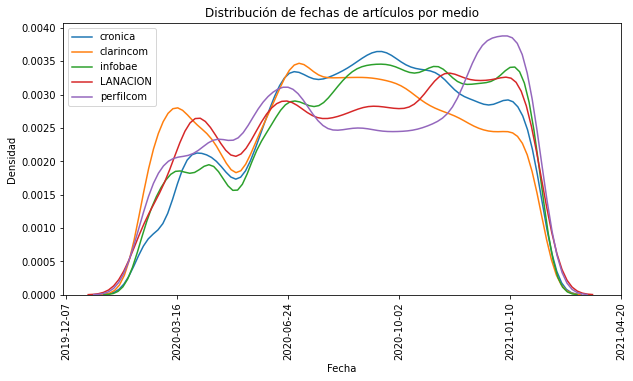
\includegraphics[width=\textwidth]{img/fechas_por_medios_todas.png}
    \caption{Distribución temporal de artículos recolectados}
    \label{fig:fecha_articulos_por_medio_todas}
    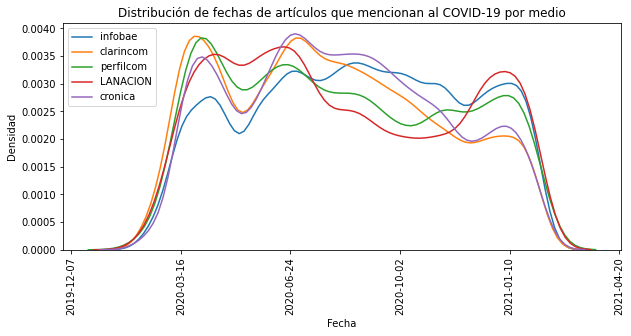
\includegraphics[width=\textwidth]{img/fechas_por_medios.png}
    \caption{Distribución temporal de artículos recolectados que mencionan COVID-19 o algún término relacionado}
    \label{fig:fecha_articulos_por_medio_covid}
\end{figure}

